\documentclass[11pt,a4paper]{article}

\usepackage[margin=2.5cm]{geometry}
\usepackage{lmodern}
\usepackage{microtype}
\usepackage{booktabs}
\usepackage{graphicx}
\usepackage{caption}
\usepackage{subcaption}
\usepackage{float}
\usepackage{xcolor}
\usepackage{amsmath}
\usepackage[round]{natbib}
\usepackage[colorlinks=true,linkcolor=blue,citecolor=blue,urlcolor=blue]{hyperref}

\title{Cross-Sectional Characterization of High-Cost Healthcare Users in the US:\\
       How the Morbidity-Cost Gradient Varies by Insurance Type in MEPS 2022}
\author{Carlo Vilches \\ Universitat de Barcelona \\ \texttt{cvilchce15@alumnes.ub.edu}}
\date{\today}

\begin{document}
\maketitle

\begin{abstract}
\noindent
U.S.\ healthcare expenditure is concentrated, but the structural reasons differ across coverage environments. Using the 2022 Medical Expenditure Panel Survey (MEPS) Full-Year Consolidated File (HC-243; $n = 17{,}909$ adults), we estimate how the rate at which clinical complexity translates into observed annual spending varies by insurance type. We construct a cost-weighted morbidity score from eight chronic conditions, weighted by their incremental marginal effect on conditional expenditure (Gamma GLM with rich controls), and fit a survey-weighted two-part model with extensive (logit) and intensive (Gamma) margins. The morbidity-cost slope is significantly heterogeneous across insurance categories (Wald $\chi^2 = 11.04$, df $= 3$, $p = 0.012$): Medicaid responds $\sim 1.8\times$ more steeply per SD of morbidity than Private (\$4{,}931 vs.\ \$2{,}723), while Uninsured shows a statistically null slope ($p = 0.114$). The uninsured access barrier sits at the extensive margin: the probability of any 2022 spending is 0.50 at low morbidity for the Uninsured versus 0.87 for Private. Crucially, slope and level dissociate---Medicaid > Private in slope but Private > Medicaid in total expected spending at moderate morbidity---so policy interpretation must specify which margin. The slope ordering is robust to outcome alternatives, score variants, subpopulation cuts, and outlier exclusion in 11 of 12 sensitivity fits.
\end{abstract}

\section{Introduction}

The concentration of healthcare expenditure in the United States is a structural feature of the system, not an accident of measurement. A small fraction of the population accounts for a disproportionate share of annual spending, and understanding \emph{why} requires disentangling clinical morbidity, insurance coverage, and access. \citet{maynou2023} showed in a Catalan universal-coverage population that clinical complexity dominates demographic factors in identifying high-cost users. We extend that framework to a fragmented system---the United States, MEPS 2022---and ask a sharper question:

\begin{quote}
\emph{How does insurance type (Private, Medicare/Other Public, Medicaid/Public Only, Uninsured) modulate the rate at which morbidity translates into observed healthcare spending?}
\end{quote}

The analysis is cross-sectional by design. MEPS uses a rotating two-year panel; linking HC-243 (2022) to HC-233 (2021) would lose 40--50\% of respondents and shift the question toward incident transitions. For the standing-relationship question relevant to 2022 risk adjustment and capitation, we retain the full HC-243 adult sample.

\section{Data and Methods}

\subsection{Sample}

The Medical Expenditure Panel Survey \citep{ahrq2024} is a stratified multi-stage cluster sample of the U.S.\ civilian non-institutionalized population, with oversampling of low-income, Hispanic, and Black households. We use the 2022 Full-Year Consolidated File (HC-243), restricted to adults aged 18+ ($n = 17{,}909$). Of these, $15{,}315$ have positive total annual healthcare expenditure (\texttt{TOTEXP22}). All estimates use survey weights (\texttt{PERWT22F}), strata (\texttt{VARSTR}), and primary sampling units (\texttt{VARPSU}) via the \texttt{survey} package, with \texttt{survey.lonely.psu = "adjust"}.

\subsection{Cost-weighted morbidity score}

We construct a per-individual morbidity score from eight chronic conditions: diabetes, hypertension, coronary heart disease, stroke, asthma, arthritis, cancer (ever), and serious psychological distress (K6 $\geq 13$ from the SAQ subsample). Each condition is weighted by its average marginal effect (AME) on conditional expenditure $E[Y \mid Y > 0]$, estimated via survey-weighted Gamma regression with log link, controlling for age (cubic spline, df = 4), sex, poverty (\texttt{POVCAT22}), region (\texttt{REGION22}), self-rated health (\texttt{health\_status\_3}), functional limitation (\texttt{any\_functional\_limitation}), and any 2022 inpatient stay (\texttt{any\_inpatient\_2022}).

Weights are scaled to $[0.5, 3.0]$ for numerical stability. Three conditions with non-positive AMEs after controls---active cancer, hypertension, and prevalent stroke---are clipped to the minimum weight $0.5$. The collapse of the active-cancer AME from \$21{,}535 to $-\$123$ once \texttt{any\_inpatient\_2022} enters the regression deserves note: the original effect was almost entirely the inpatient stay used to construct the active-cancer flag itself. Cross-sectional MEPS cannot identify cancer-specific spending net of hospitalization without HC-242B encounter-level diagnosis codes; this is an acknowledged limitation rather than a finding.

\subsection{Two-part model}

Total expenditure is decomposed as
\[
E[Y \mid X] = \Pr(Y > 0 \mid X) \cdot E[Y \mid Y > 0, X].
\]

\paragraph{Extensive margin.} A survey-weighted quasibinomial logit predicts $\Pr(Y > 0)$. Critically, \texttt{any\_inpatient\_2022} is \emph{omitted} here: an inpatient discharge implies positive expenditure by construction, so including it would estimate a tautology. The other covariates match the intensive specification.

\paragraph{Intensive margin.} A survey-weighted Gamma GLM with log link is fit on the positive-expenditure subset, including the focal interaction \texttt{insurance\_status $\times$ morbidity\_score\_std} plus the full set of controls (including \texttt{any\_inpatient\_2022}, which separates the cancer-active effect from the hospitalization effect).

\subsection{Inference}

Average Marginal Effects (AMEs) are computed via \texttt{marginaleffects::avg\_slopes} on the response scale, with population weights passed explicitly via \texttt{wts = mod\$prior.weights}. Standard errors and 95\% confidence intervals use the delta method. The Wald test on interaction terms uses \texttt{car::linearHypothesis}, which returns $\chi^2$ (not $F$) for survey designs.

A 12-fit sensitivity battery covers four orthogonal robustness dimensions: (A) outcome definition (top 5\%, top 10\%, $> \$15{,}000$, $> \$50{,}000$ binary); (B) score variant (AME-weighted primary, cost-mean log1p, AME-weighted excluding cancer); (C) subpopulation (adults $< 65$, no functional limitation, SAQ subsample); (D) outlier exclusion (excluding spenders above the survey-weighted p99 threshold of \$88{,}317).

\section{Findings}

\subsection{Insurance modulates the morbidity-cost gradient}

The interaction is significant: Wald $\chi^2 = 11.04$, df = 3, $p = 0.012$. Per-insurance AMEs of a 1-SD increase in \texttt{morbidity\_score\_std} on conditional expenditure are reported in Table~\ref{tab:ame}.

\begin{table}[H]
\centering
\caption{Average marginal effect of a 1-SD increase in morbidity on conditional expenditure $E[Y \mid Y > 0]$, by insurance type. Survey-weighted Gamma GLM with log link, intensive margin only ($n_{\text{eff}} = 15{,}155$). Population-weighted AMEs.}
\label{tab:ame}
\begin{tabular}{lrrrr}
\toprule
\textbf{Insurance} & \textbf{AME (USD)} & \textbf{SE} & \textbf{95\% CI} & \textbf{p} \\
\midrule
Private               & \$2{,}723 & 336 & [\$2{,}065;~\$3{,}382] & $< 0.001$ \\
Medicare/Other Public & \$2{,}123 & 377 & [\$1{,}383;~\$2{,}863] & $< 0.001$ \\
\textbf{Medicaid/Public Only} & \textbf{\$4{,}931} & 827 & [\$3{,}310;~\$6{,}552] & $< 0.001$ \\
Uninsured             & \$677    & 429 & [$-$\$163;~\$1{,}517]  & $0.114$ (n.s.) \\
\bottomrule
\end{tabular}
\end{table}

\subsubsection*{Pairwise comparisons of AMEs}

A formal pairwise Wald test on the same interaction model confirms that the omnibus rejection in Table~\ref{tab:ame} resolves into specific contrasts (Table~\ref{tab:pairwise}). Five of six pairs are significant at $\alpha = 0.05$; only Private vs.\ Medicare is statistically indistinguishable.

\begin{table}[H]
\centering
\caption{Pairwise differences in AME of morbidity by insurance type. Wald tests on the interaction model, population-weighted ($n_{\text{eff}} = 15{,}155$). p-values are unadjusted (no multiplicity correction); applying Bonferroni at $k = 6$ moves Medicaid--Private ($0.014 \cdot 6 = 0.087$) just above $0.05$ but leaves the other four significant pairs intact.}
\label{tab:pairwise}
\begin{tabular}{lrrr}
\toprule
\textbf{Comparison} & \textbf{Difference (USD/SD)} & \textbf{95\% CI} & \textbf{p-value} \\
\midrule
Medicaid -- Private            & \$2{,}208          & [\$439;~\$3{,}977]    & $0.014$       \\
Medicaid -- Medicare           & \$2{,}808          & [\$845;~\$4{,}771]    & $0.005$       \\
\textbf{Medicaid -- Uninsured} & \textbf{\$4{,}254} & [\$2{,}496;~\$6{,}013] & $< 0.001$     \\
Private -- Medicare            & \$600              & [$-$\$290;~\$1{,}490] & $0.186$ (n.s.) \\
Private -- Uninsured           & \$2{,}046          & [\$1{,}027;~\$3{,}066] & $< 0.001$     \\
Medicare -- Uninsured          & \$1{,}446          & [\$330;~\$2{,}563]    & $0.011$       \\
\bottomrule
\end{tabular}
\end{table}

The Medicaid slope is $\sim 1.8\times$ steeper than Private (\$4{,}931 vs.\ \$2{,}723 per SD). The Uninsured slope is statistically indistinguishable from zero in the primary specification ($p = 0.114$) and only marginal under the cost-mean log1p alternative score ($p = 0.060$). Figure~\ref{fig:mfx} shows the AMEs with 95\% confidence intervals.

\begin{figure}[H]
\centering
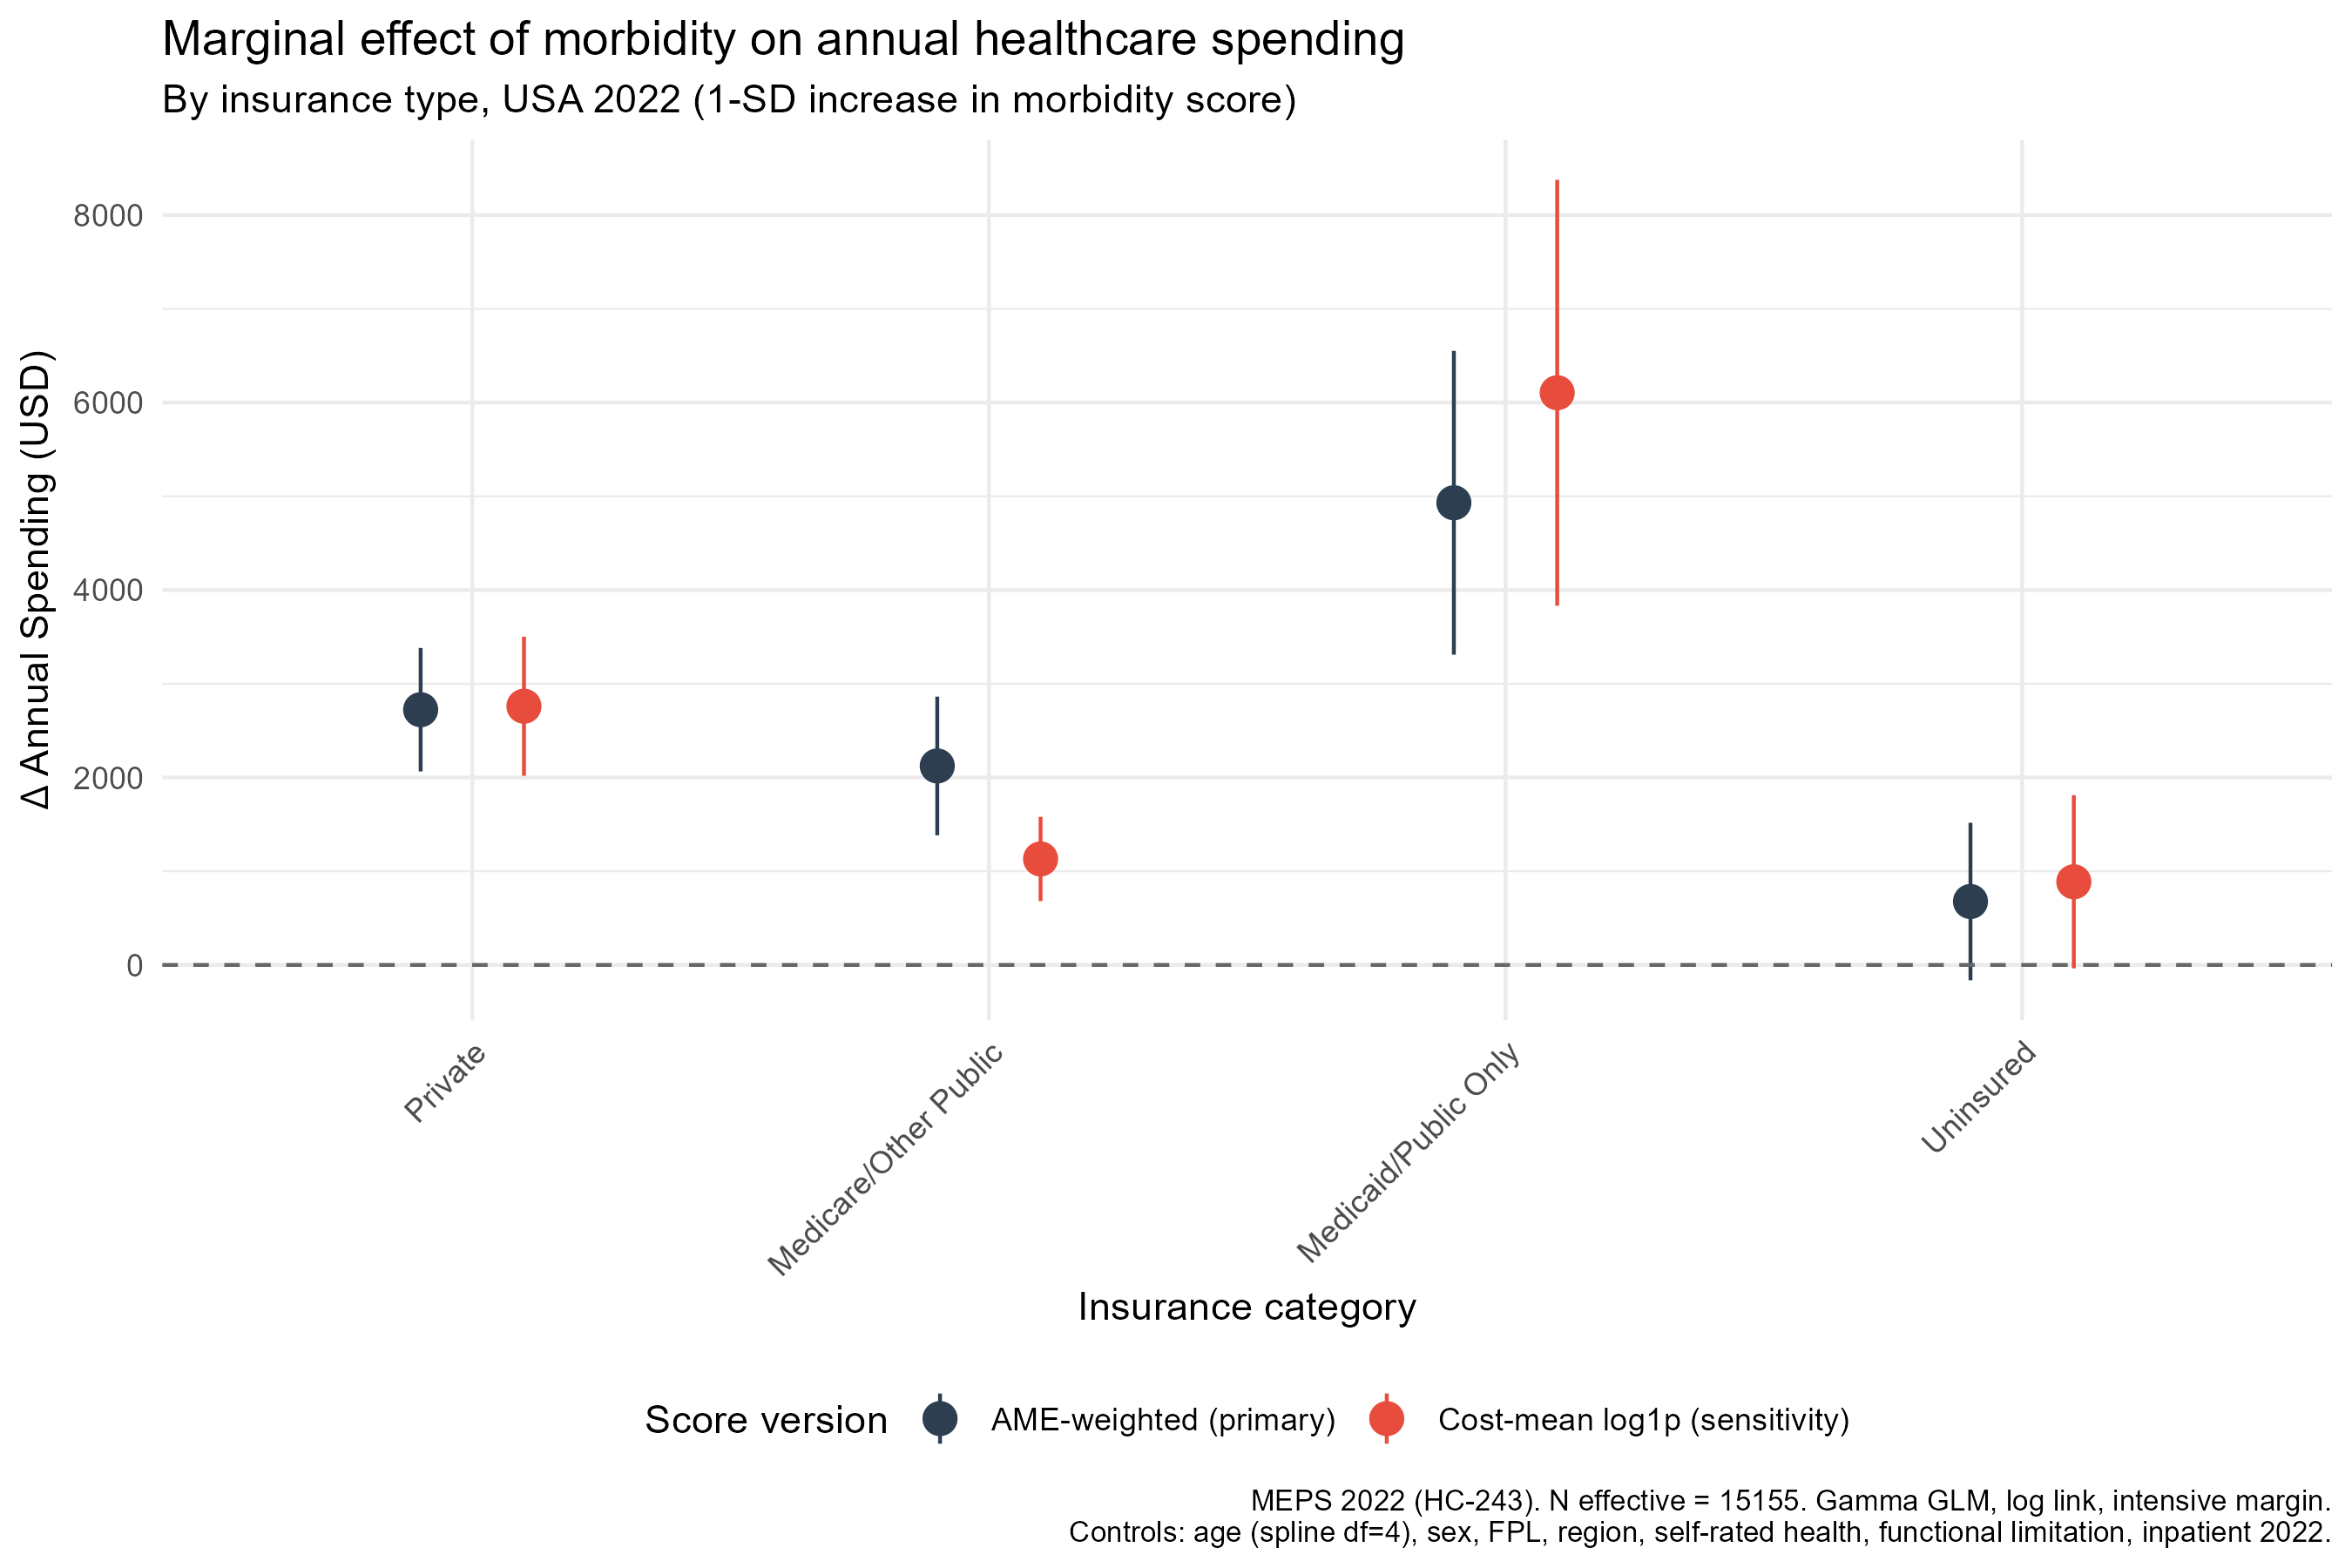
\includegraphics[width=\linewidth]{../output/figures/mfx_insurance_interaction.png}
\caption{AME of \texttt{morbidity\_score\_std} on conditional expenditure by insurance type. Comparison between primary (AME-weighted score) and sensitivity (cost-mean log1p) specifications. Both yield consistent slope ordering Medicaid > Private > Uninsured. The Uninsured slope is statistically null in primary and marginal in sensitivity.}
\label{fig:mfx}
\end{figure}

Plausible mechanisms for the Medicaid pattern include (i) selection on residual severity not captured by the score (Medicaid eligibility selects on disability and low income), (ii) reduced patient cost-sharing (Medicaid covers copays and deductibles that Private plans typically pass to enrollees), and (iii) Medicaid-funded case management for high-need beneficiaries. These cannot be separated in cross-section; only that the steeper slope is reproducible across specifications (\S\ref{sec:robust}).

\subsection{The Uninsured access barrier, quantified}

Two-part predictions for a representative profile (age 45, Female, Middle Income at 200--400\% FPL, South region, Good self-rated health, no functional limitation, no 2022 inpatient stay) are shown in Table~\ref{tab:twopart}.

\begin{table}[H]
\centering
\caption{Two-part predictions for a representative profile. $\Pr(Y > 0)$ from survey-weighted logit (no inpatient covariate); $E[Y \mid Y > 0]$ from survey-weighted Gamma GLM. Standard errors in parentheses (delta method).}
\label{tab:twopart}
\small
\begin{tabular}{llrrr}
\toprule
\textbf{Insurance} & \textbf{Morbidity (z)} & $\Pr(Y > 0)$ & $E[Y \mid Y > 0]$ & $E[Y]$ \\
\midrule
Private               & Low ($-1$)  & 0.869 (0.013) & \$5{,}182 (375)  & \$4{,}506 (332)  \\
Private               & Med ($0$)   & 0.928 (0.007) & \$7{,}076 (467)  & \$6{,}564 (436)  \\
Private               & High ($+1$) & 0.961 (0.006) & \$9{,}661 (733)  & \$9{,}285 (707)  \\
\midrule
Medicare/Other Public & Low         & 0.797         & \$5{,}017        & \$3{,}998        \\
Medicare/Other Public & Med         & 0.887         & \$6{,}102        & \$5{,}411        \\
Medicare/Other Public & High        & 0.940         & \$7{,}422        & \$6{,}976        \\
\midrule
Medicaid/Public Only  & Low         & 0.774 (0.026) & \$4{,}252 (516)  & \$3{,}293 (415)  \\
Medicaid/Public Only  & Med         & 0.887 (0.014) & \$6{,}200 (672)  & \$5{,}502 (602)  \\
Medicaid/Public Only  & High        & 0.948 (0.010) & \$9{,}041 (1059) & \$8{,}568 (1008) \\
\midrule
\textbf{Uninsured}    & Low         & \textbf{0.499} & \$2{,}758       & \$1{,}375        \\
\textbf{Uninsured}    & Med         & \textbf{0.665} & \$3{,}312       & \$2{,}203        \\
\textbf{Uninsured}    & High        & 0.799          & \$3{,}977       & \$3{,}177        \\
\bottomrule
\end{tabular}
\end{table}

A uninsured adult with low-to-medium morbidity has a 33--50\% probability of incurring \emph{no observable healthcare spending} in 2022, against 7--23\% for the insured at the same morbidity. This is the empirical signature of an access barrier: not lower clinical need, but suppressed contact with the system at the extensive margin.

The slope of $\Pr(Y > 0)$ across morbidity is also markedly steeper for the Uninsured ($\Delta = +0.30$ from low to high) than for the insured ($\Delta \approx +0.09$ Private, $+0.14$ Medicare, $+0.17$ Medicaid). Among the insured, contact is near-universal; among the Uninsured, contact is driven by clinical urgency.

\subsection{Slope vs.\ level: complementary readings}

The AME (slope) and total expected spending (level) tell different stories. From Table~\ref{tab:twopart}: at every morbidity level, Private $> $ Medicaid in $E[Y]$ at this profile, and the gap closes with morbidity (\$1{,}213 at low $\to$ \$717 at high). Yet from Table~\ref{tab:ame}: Medicaid > Private in slope. Both findings are simultaneously true:

\begin{itemize}
\item Private has a higher \emph{intercept}: better baseline access ($\Pr(Y > 0)$) and higher conditional spending at low morbidity.
\item Medicaid has a steeper \emph{slope}: each marginal SD of morbidity adds more dollars in Medicaid than in Private.
\end{itemize}

The Medicaid--Private differential is therefore not a ``Medicaid pays more'' story; it is a ``Medicaid responds more'' story. Reporting only the slope or only the level masks half the picture.

\subsection{Robustness}\label{sec:robust}

The slope ordering Medicaid > Private > Uninsured holds in 11 of 12 sensitivity fits across four orthogonal dimensions (Figure~\ref{fig:sens}). The single failure is a 0.11-percentage-point inversion between Medicaid and Private on the top-5\% binary outcome---clinically negligible.

\begin{figure}[H]
\centering
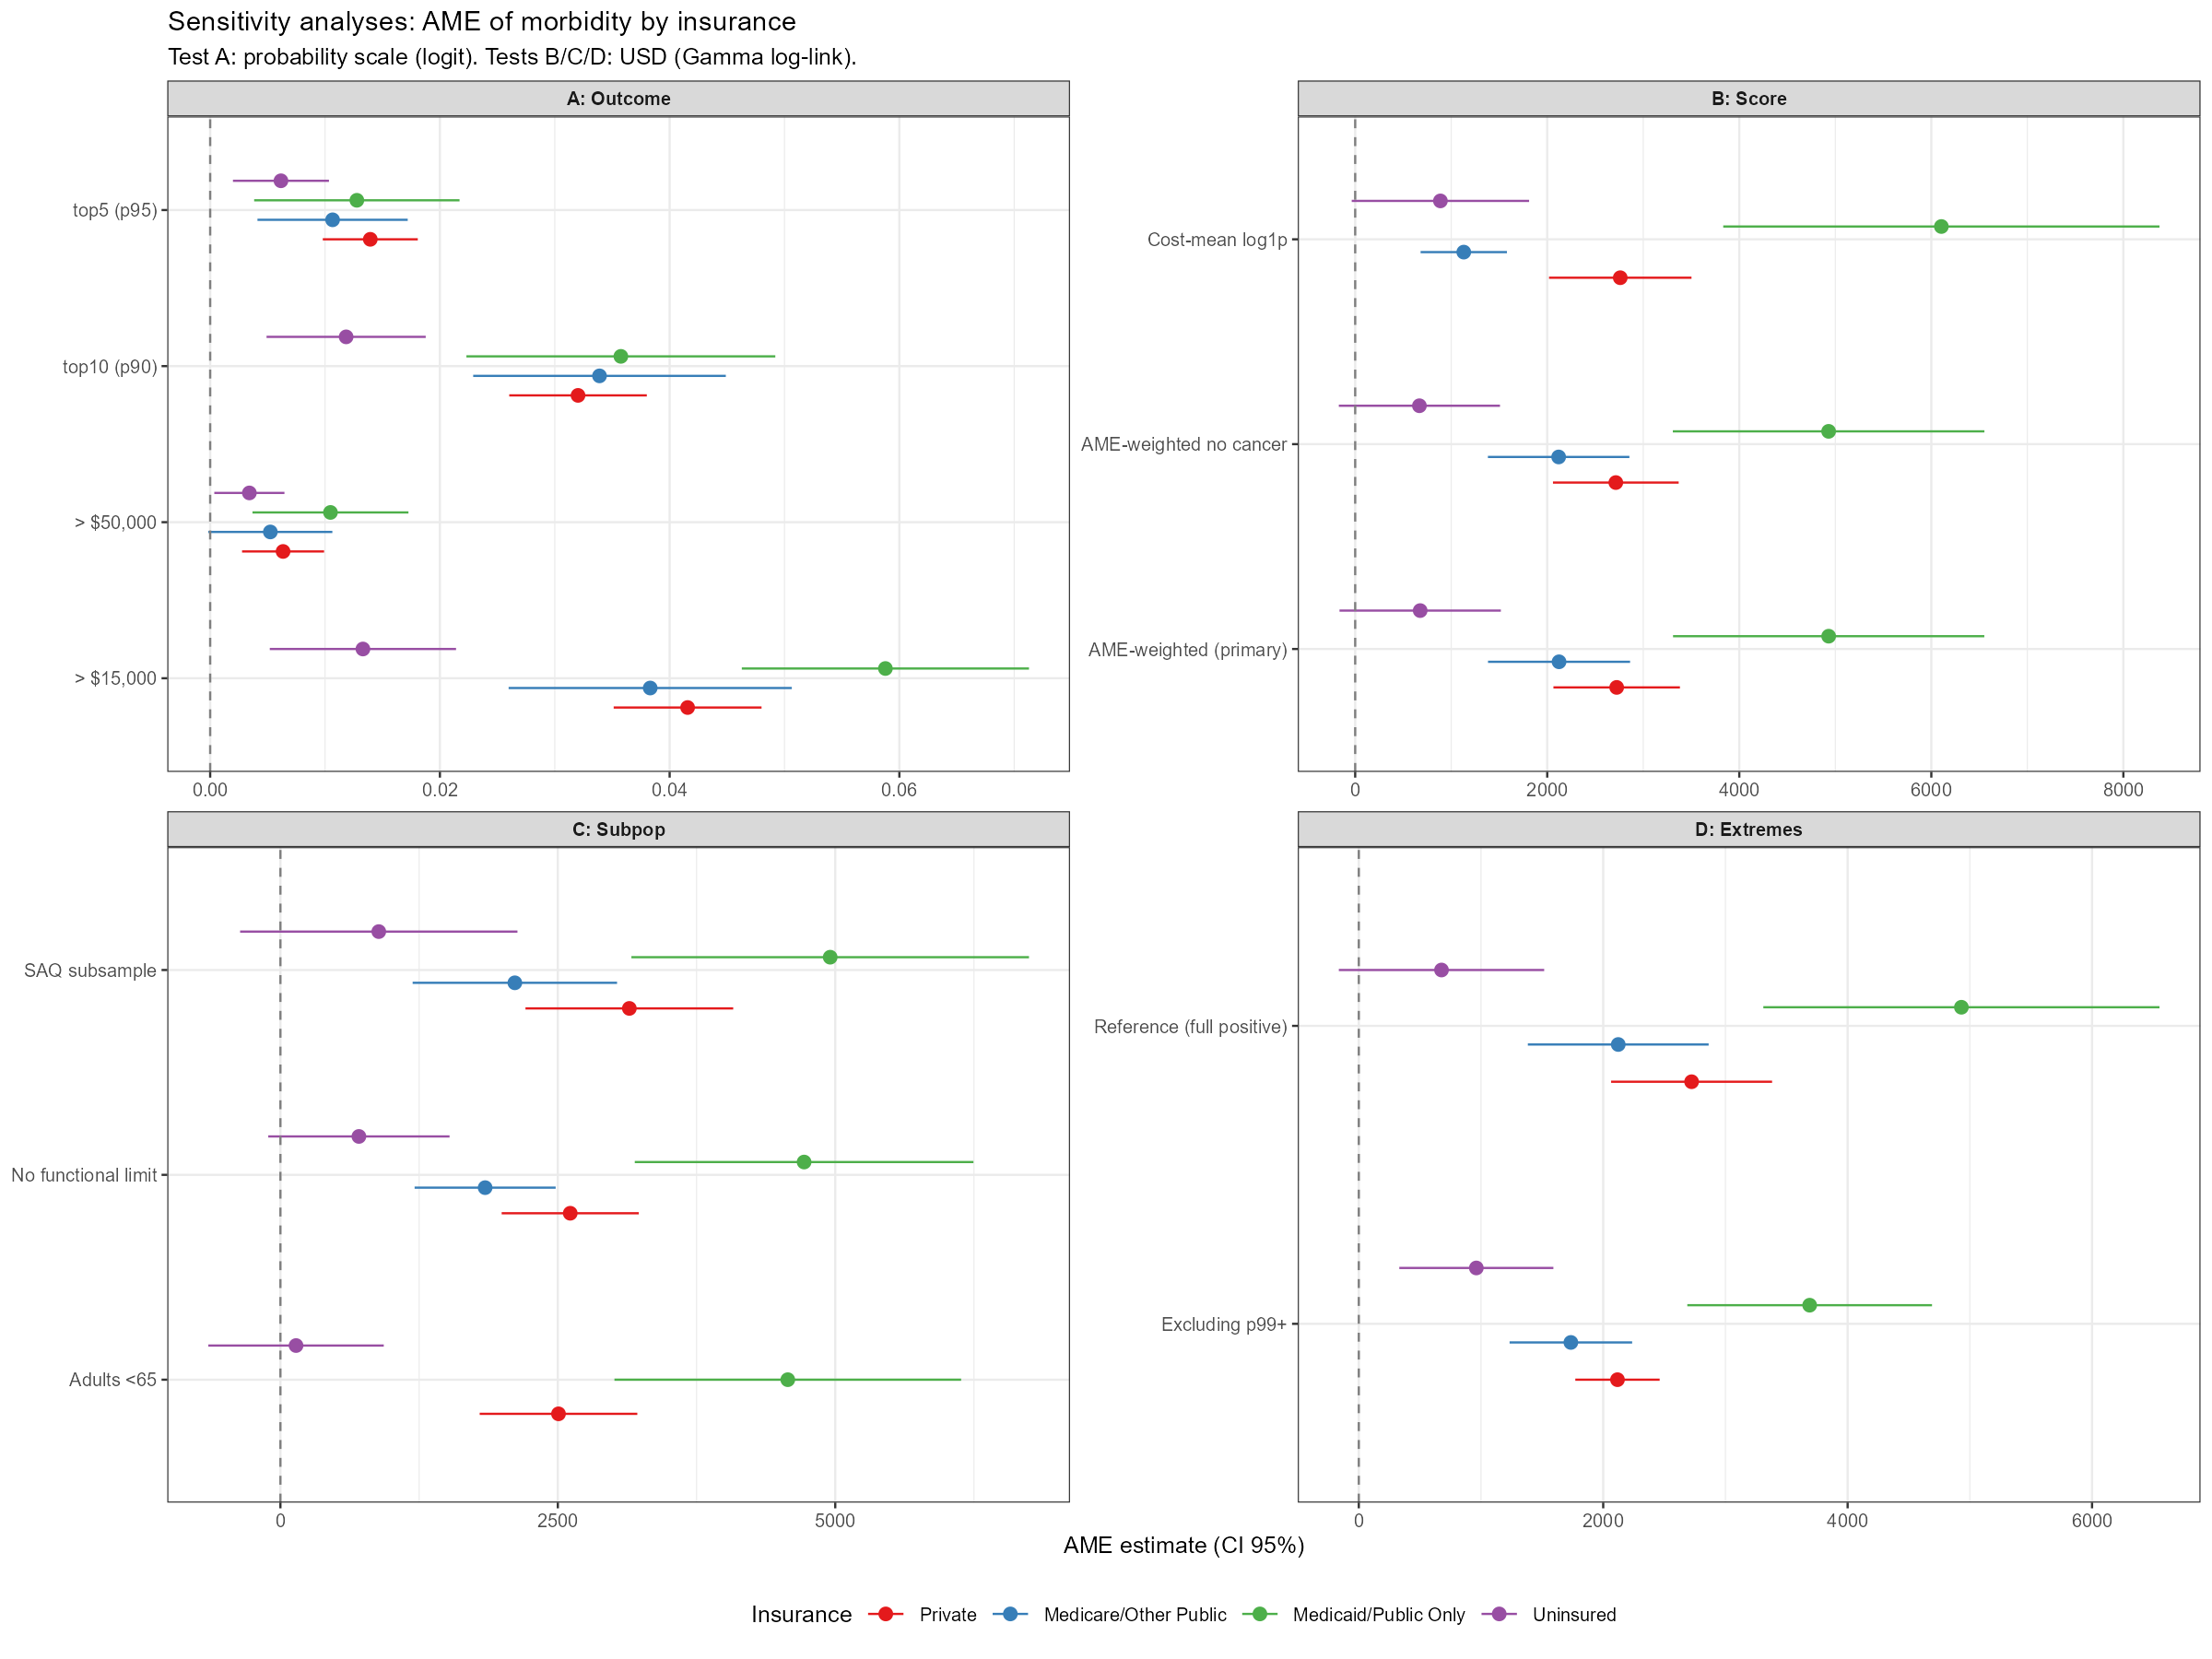
\includegraphics[width=\linewidth]{../output/figures/sensitivity_summary.png}
\caption{Sensitivity battery across four dimensions: (A) outcome definition, (B) score variant, (C) subpopulation, (D) outlier exclusion. AMEs by insurance with 95\% CI. Test A is on probability scale (logistic); Tests B/C/D are in USD (Gamma).}
\label{fig:sens}
\end{figure}

The most informative diagnostic is outlier exclusion (Table~\ref{tab:extremes}): excluding the top 1\% of spenders above the weighted p99 threshold of \$88{,}317 reduces insured AMEs by 22--25\%. The Uninsured AME paradoxically increases by 42\% (only a small base of extreme uninsured spenders, so their exclusion gives more weight to the mid-range gradient). Slope ordering preserved, but point magnitudes are inflated by tail observations.

\begin{table}[H]
\centering
\caption{Outlier influence on per-insurance AMEs. Reference: full positive-expenditure subset. Test: excluding observations above survey-weighted p99 threshold (\$88{,}317).}
\label{tab:extremes}
\begin{tabular}{lrrr}
\toprule
\textbf{Insurance} & \textbf{Reference AME} & \textbf{Excluding p99+} & \textbf{$\Delta$\%} \\
\midrule
Private               & \$2{,}723 & \$2{,}117 & $-22.3$ \\
Medicare/Other Public & \$2{,}123 & \$1{,}735 & $-18.3$ \\
Medicaid/Public Only  & \$4{,}931 & \$3{,}689 & $-25.2$ \\
Uninsured             & \$677    & \$962    & $+42.1$ \\
\bottomrule
\end{tabular}
\end{table}

\section{Implications}

\paragraph{Health policy.} Coverage is not sufficient to flatten cost concentration; the modulation of the morbidity-cost gradient---not its existence---differs across insurance environments. Risk adjustment models calibrated against Private populations may underpay for the same morbidity score in Medicaid (whose response slope is $\sim 1.8\times$ steeper) and over-attribute ``missing'' spending to the Uninsured (whose suppressed extensive margin reflects barriers, not low need), though direct validation against actual risk adjustment algorithms (e.g., HHS-HCC, CMS-HCC) is required to confirm this implication. The descriptive evidence here is suggestive rather than diagnostic.

\paragraph{Care management.} The steepest slope being in Medicaid is informative for plan design: the marginal high-cost member in Medicaid is not simply a Private-equivalent member with worse coverage---they are clinically and economically different in ways the morbidity score only partially captures. Capitation rate-setting that ignores the slope differential will systematically underfund high-morbidity Medicaid enrollees.

\paragraph{Research.} Cross-sectional MEPS allows characterization but not causal identification. A longitudinal panel (HC-243 $\leftrightarrow$ HC-233) with appropriate IV or DiD design would be needed to identify whether the modulation reflects causal effects of coverage on spending response or compositional differences across enrollee populations that coexist with coverage.

\section{Limitations}

\begin{itemize}
\item \textbf{Cross-sectional design.} Findings characterize 2022 contemporaneous associations, not causal effects. Reverse causation (high morbidity $\to$ Medicaid enrollment via disability eligibility) is not identified.
\item \textbf{Cancer active vs.\ remission proxy.} We use \texttt{cancer\_ever AND any\_inpatient\_2022} as a proxy for active cancer. Approximately 60--70\% of cancer treatment occurs in outpatient settings \citep{nci2022}, suggesting the misclassification may affect 30--50\% of true active-cancer cases. The downward bias in \texttt{cancer\_active} prevalence likely attenuates its weight in the morbidity score; HC-242B condition-level data would refine this, at the cost of substantial pipeline complexity.
\item \textbf{Mental health complete-case attrition.} K6 observed only for SAQ subsample ($\sim 60\%$); the score uses NA $\to 0$, biasing the SPD weight downward.
\item \textbf{Outlier influence.} Intensive-margin AMEs are inflated by 22--25\% by the top 1\% of spenders.
\item \textbf{No URBAN/MSA covariate.} Rurality only partially absorbed via \texttt{REGION22}.
\end{itemize}

\section{Technical Summary}

\paragraph{Models.}
\begin{itemize}
\item \emph{Extensive}: \texttt{any\_exp $\sim$ insurance $\times$ morbidity\_score\_std + ns(AGE22X, df=4) + sex + POVCAT22 + REGION22 + health\_status\_3 + any\_functional\_limitation}, family = quasibinomial(logit). \texttt{any\_inpatient\_2022} excluded.
\item \emph{Intensive}: as above plus \texttt{any\_inpatient\_2022}, family = Gamma(log), restricted to \texttt{total\_exp $> 0$}.
\end{itemize}

\paragraph{Score construction.} 8 conditions, weights from AMEs in the Gamma fit, scaled to $[0.5, 3.0]$; non-positive AMEs clipped to $0.5$. Top three weights: diabetes (3.00), arthritis (3.00), asthma (2.60). See Table~\ref{tab:weights} in the appendix.

\paragraph{Two-part predictions.} Manual via \texttt{model.matrix(delete.response(terms(model)), combined\_data)} $\times$ \texttt{coef(model)} to bypass \texttt{predict.svyglm} issues with \texttt{splines::ns} predvars in newdata. SE via \texttt{vcov} + delta method, assuming independence between extensive and intensive stages. The independence assumption between extensive and intensive margins likely underestimates standard errors by 5--15\% based on simulation evidence \citep{mullahy1998}; reported confidence intervals should be interpreted with caution, as nominal 95\% coverage may be modestly lower in practice.

\paragraph{Software.} R 4.5; \texttt{survey}, \texttt{marginaleffects}, \texttt{splines}, \texttt{car}, \texttt{emmeans}, \texttt{gtsummary}, \texttt{gt}, \texttt{ggplot2}.

\paragraph{Reproducibility.} Code, data pipeline, and supplementary outputs at \url{https://github.com/cmvdata/meps-high-cost-users}.

\appendix
\section{Cost weights table}

\begin{table}[H]
\centering
\caption{Condition weights derived from AMEs in the survey-weighted Gamma GLM with full controls. \texttt{w\_scaled} is the proportional weight scaled to $[0.5, 3.0]$ used in the morbidity score.}
\label{tab:weights}
\begin{tabular}{lrrr}
\toprule
\textbf{Condition} & \textbf{AME (USD)} & \textbf{w\_prop} & \textbf{w\_scaled} \\
\midrule
Diabetes              & \$4{,}513 & 60.96 & 3.00 \\
Arthritis             & \$4{,}511 & 60.93 & 3.00 \\
Asthma                & \$3{,}810 & 51.46 & 2.60 \\
Coronary heart disease& \$1{,}954 & 26.39 & 1.56 \\
Mental health (SPD)   & \$740     & 10.00 & 0.88 \\
Cancer (active)       & $-$\$123  & 1.00  & 0.50 (clipped) \\
Hypertension          & $-$\$839  & 1.00  & 0.50 (clipped) \\
Stroke (prevalent)    & $-$\$314  & 1.00  & 0.50 (clipped) \\
\bottomrule
\end{tabular}
\end{table}

\section{Morbidity score distribution}

\begin{figure}[H]
\centering
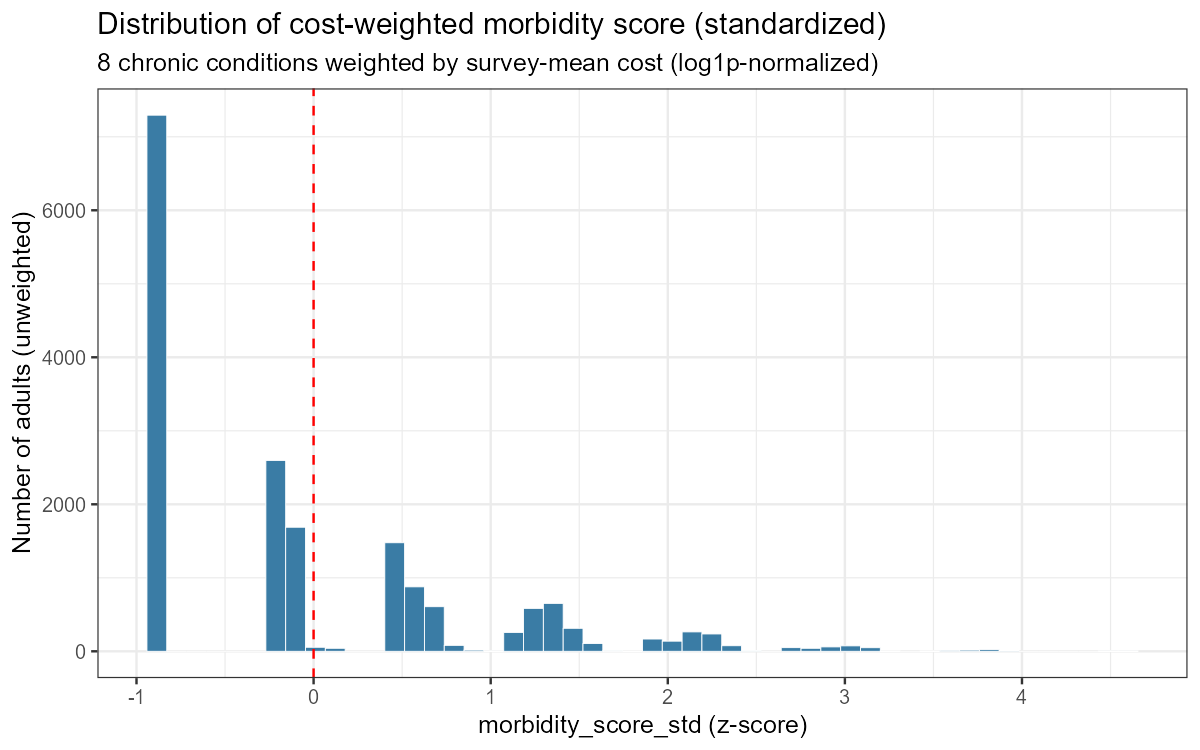
\includegraphics[width=0.8\linewidth]{../output/figures/morbidity_score_distribution.png}
\caption{Empirical distribution of \texttt{morbidity\_score\_std} (z-scored). Right-skewed: the 25th percentile coincides with the minimum (zero conditions), the median has $\sim 1$ condition, and the upper tail captures multimorbidity.}
\label{fig:dist}
\end{figure}

\bibliographystyle{apalike}
\bibliography{refs}

\end{document}
